% !TeX root = ../../main.tex
% chapters/3_cbic/method.tex -- one section of Chapter 3 (CBIC 2025, published).
% Split out of chapters/3_cbic.tex on 2026-07-28 (author request: the paper
% chapters were single long files, while the originals under articles/CBIC___MTL/sections/
% are one file per section). The split is PURELY MECHANICAL: content was cut at
% \section boundaries and not edited. The chapter file now \inputs these in order.
% Editing rules are unchanged and still governed by the chapter's status above:
% see NORTH_STAR section 4 before changing any sentence here.
\section{Methodology}
\label{sec:cbic:methodology}

This section details the proposed methodology for Point-of-Interest (POI) category classification and next-POI prediction using a MTL approach. We first describe the generation of POI embeddings and the preparation of data for both tasks. Subsequently, we present the architectures of the single-task baselines, which are also used as task-specific heads within our MTL framework. Finally, we elaborate on the proposed MTL architecture, including the hard parameter-sharing strategy and the Nash-MTL optimizer employed for gradient aggregation.

\subsection{POI Embeddings and Data Preparation}
\label{sec:cbic:embeddings}

This chapter computes POI embeddings using graph attention convolution along with contrastive learning based on Deep Graph Infomax (DGI). These embeddings are the input for the MTL model discussed in Section~\ref{sec:cbic:mtlarch}.

\subsubsection{POI Embeddings}

A point of interest is defined as a tuple $\langle id, lat, long, cat \rangle$, where $id$ serves as a unique identifier, $lat$ and $long$ represent its coordinates, and $cat$ denotes its category, such as restaurant or pharmacy. A place suffers from complementarity effect \cite{du2019beyond}, implying that a location is affected by its neighbors (e.g. leisure zones are often near residential districts). Hence, we propose a graph-based contrastive method to capture this spatial locality behavior, generating a POI embedding to serve as input to our MTL model.

To capture the spatial locality and capture neighborhood information, we model the weighted graph $G(V, E)$ as a Delaunay Triangulation, where each vertex $v \in V$ represents a POI and edge $e_{ij} \in E$ defines the connection between POI $p_i$ and a POI $p_j$. Besides that, following \cite{huang2022estimating} the weight of an edge $e_{ij}$ is defined as $w_{ij} = \log((1+D^{1.5}/1+d_{ij}^{1.5}))$, where D is the diagonal length of bounding box that encloses the coordinates of POIs, and $d_{ij}$ is the geodesic distance between $p_{i}$ and $p_{j}$. The node feature matrix is based on category one-hot encoding of each POI, represented by $X \in \mathbb{R}^{n_c}$, where $n_c$ is the number of possible categories.\footnote{The released implementation feeds the network the mean of the one-hot vectors of a POI's graph neighbors, with the POI's own vector excluded, rather than the POI's own one-hot vector (\texttt{research/embeddings/dgi/preprocess.py}), a departure from the published description. The distinction matters for how the embedding should be read: the input describes a POI's neighborhood, so the static task the embedding supports is spatial homophily rather than recall of the POI's own label.}
% [round9, register track] "neighbours"/"neighbourhood" -> "neighbors"/"neighborhood". BRITISH, and
% WRITING_LAW §1 requires American spelling; the gate is src_utils/check_register.py. This footnote is
% NOT published prose: measured, neither string occurs anywhere in articles/CBIC___MTL/sections/*.tex
% (which has no "released implementation" text at all), so no errata row is owed. The published
% sentence this footnote annotates is untouched, and it already writes "neighbors" American at
% line 21 of this file -- the footnote was the only British spelling in the file.
% [round5, cross-check finding] The published sentence is preserved; the footnote records what the
% released code does. Verified: dgi.py:56 sets x=embedding_array_test, and preprocess.py:121-130
% builds that as the neighbour mean with the node itself excluded (isolated nodes get a zero vector).
% This is the distinction that refutes the "Ch.3 has direct target leakage" reading.

Therefore, to encode the Delaunay graph we apply a graph attention convolution layer \cite{velivckovic2017graph}, yielding an embedding $h_i \in \mathbb{R}^{d}$, where $d$ is the dimension of the output. In addition, we utilize a Deep Graph Infomax (DGI) \cite{velickovic2019deep} as a contrastive learning method to maximize the mutual information between local representations (node embeddings) and the global graph embedding compared to a corrupted version of a graph, which is guided by the Equation~\ref{eq:cbic:loss}.
%
\begin{equation}
  \mathcal{L}
  = \frac{1}{2|V|}\Bigl(
        \sum_{i=1}^{|V|}
          \mathbb{E}_{(X,G)}
          [\log \mathcal{D}(\vec{h}_i,\vec{s})]
        +
        \sum_{j=1}^{|V|}
          \mathbb{E}_{(\tilde{X}, G)}
          [\log (1-\mathcal{D}(\tilde{\vec{h}}_j,\vec{s}))]\Bigr)
  \label{eq:cbic:loss}
\end{equation}
%
where $X$ and $G$ denote the positive samples for the node feature matrix and graph adjacency, respectively, while $\tilde{X}$ is the corrupted version of the feature matrix. To corrupt the features, we employ a random shuffling method. Additionally, $\vec{s}$ is the global graph embedding derived by applying global mean pooling to the embedding matrix $H = [h_i, h_{i+1}, \ldots, h_{n}]$ in our model. In addition, $\mathcal{D}$ is a discriminator that differentiates each positive example from its corrupted version, learning from their dissimilarities; in our POI Embedding, this discriminator is implemented as a linear model.

\subsubsection{Data Processing for POI Category Classification}
Each POI is represented by its 64-dimensional DGI embedding $\mathbf{e}\!\in\!\mathbb{R}^{64}$.
The dataset therefore consists of pairs $(\mathbf{e},\,c)$, where $c$ is the POI's ground-truth category to be predicted.

\subsubsection{Data Processing for Next-POI Category Prediction}
This task predicts the category of the next POI a user will visit from their recent check-in history.

\begin{enumerate}
  \item \textbf{Trajectory building.}  Check-ins (user, POI, timestamp) are ordered chronologically per user; users with fewer than five visits are discarded.
  \item \textbf{Sequence extraction.}  From each trajectory we draw non-overlapping windows of length $L_h\!=\!9$: $(p_1,\dots,p_9)$ as context and $p_{\text{target}}$ as the next POI.
  \item \textbf{Feature/label construction.}
    \begin{itemize}
      \item The input is the concatenation of the 64-dimensional embeddings of $p_1$--$p_9$, yielding a $9\!\times\!64=576$-dim vector.
            Histories shorter than nine are padded by a special POI whose embedding is $\mathbf{0}$.
      \item The label is the category of $p_{\text{target}}$.
    \end{itemize}
\end{enumerate}

This format allows the model to infer the category of the next POI solely from the embeddings of the previous visits.

\subsection{Multitask Learning Architecture}
\label{sec:cbic:mtlarch}

Our proposed Multitask Learning (MTL) architecture, depicted in Figure~\ref{fig:cbic:arch}, is built upon a hard parameter-sharing scheme for the joint training of POI Category Classification and Next-POI Prediction. This design integrates Feature-wise Linear Modulation (FiLM) layers to condition the shared representations, a technique aimed at modulating task interactions and mitigating negative transfer \cite{perez2018film,standley2020tasks}.

\paragraph*{Architecture Overview}
Input features for POI Category Classification ($\mathbf{x}^{(c)}$) and Next-POI Prediction ($\mathbf{x}^{(n)}$) are first processed by separate, task-specific encoders. These encoders, implemented as MLPs, map the raw input features into a shared latent space of dimension $d_{\mathrm{shared}}$.

\paragraph*{Feature-wise Linear Modulation (FiLM)}
To allow for task-specific adaptation within the shared pathway, we employ FiLM layers \cite{perez2018film}. A unique, learnable task embedding $\mathbf{e}_{t}$ for each task $t$ is used to generate a scaling vector $\gamma_{t}$ and a shifting vector $\beta_{t}$. These vectors modulate the encoded features $\mathbf{h}_{\mathrm{enc}}^{(t)}$ from each task-specific encoder:
$$
\mathrm{FiLM}(\mathbf{h}_{\mathrm{enc}}^{(t)} \,|\, \mathbf{e}_{t}) = \gamma_{t} \odot \mathbf{h}_{\mathrm{enc}}^{(t)} + \beta_{t}
$$
This lightweight operation conditions the features before they enter the fully shared layers of the network.

\paragraph*{Shared Processing Layers}
The FiLM-modulated representations are processed by a sequence of shared layers. This module begins with a linear transformation followed by a LeakyReLU activation, LayerNorm, and dropout, and continues through $L_{\mathrm{shared}}$ residual blocks. This hard parameter-sharing approach regularizes the model by forcing it to learn a common, robust feature representation for both tasks \cite{baxter2000model}.

\paragraph*{Task-Specific Heads}
Finally, the processed shared representations are passed to dedicated, unshared task-specific heads. These heads generate the final predictions for each task, allowing for specialized output generation and isolated gradient computation during backpropagation.

\paragraph*{Rationale for Hard Parameter Sharing}
The choice of hard parameter sharing is motivated by its efficiency and regularization benefits, which are critical for our target application. This approach is supported by several factors:
\begin{itemize}
    \item \textbf{Computational Efficiency:} Unlike soft-sharing methods that often introduce task-specific parameters and increase computational overhead, hard sharing maintains a compact model. This is crucial for deployment on resource-constrained edge devices (e.g., NVIDIA Jetson platforms).
    \item \textbf{Implicit Regularization:} By constraining the hypothesis space, hard sharing acts as a regularizer, often leading to more generalizable models, especially when tasks are related \cite{baxter2000model}. Seminal work by Caruana demonstrated significant error reduction with this approach \cite{caruana1997multitask}.
% [round9c, PENDENCIAS_RESOLVIDOS 2.15 (arquivado 2026-08-02), author decision: path A, 2026-07-30] CITATION SUBSTITUTED,
% ruder2017sluice -> baxter2000model. Errata row in Appendix B, and the same substitution is applied
% to the published source at articles/CBIC___MTL/sections/method.tex, per the author's instruction to
% modify the original articles as well.
% WHY THE OLD KEY DOES NOT SUPPORT THE SENTENCE. Ruder et al. is a SOFT-sharing method whose
% contribution is learning what and how much to share, presented as an improvement ON fixed sharing,
% so it is evidence against the bullet it was attached to rather than for it. Title of record at
% arXiv:1705.08142 is "Latent Multi-task Architecture Learning", not the "Sluice Networks" title the
% .bib carried.
% WHY THE NEW KEY DOES. Baxter, "A Model of Inductive Bias Learning", JAIR 12:149-198, 2000,
% DOI 10.1613/jair.731, VERIFIED AT CROSSREF THIS SESSION (title, four-field attribution, volume,
% pages and year read from the record, not retyped from another bibliography). Its abstract states
% the hypothesis-space argument this bullet makes: the problem is "how to choose a learner's
% hypothesis space so that it is large enough to contain a solution ... yet small enough to ensure
% reliable generalization", and within an environment of related tasks "it can search for a
% hypothesis space that contains good solutions to many of the problems". That is constraint of the
% hypothesis space, generalization, and relatedness: the bullet's three elements.
% The key was ALREADY in the bibliography and is ALREADY cited for this same claim at
% chapters/3_cbic/method.tex:88 and chapters/4_courb/methodology.tex:32, so no bib entry is added.
% ruder2017sluice REMAINS CITED, correctly, at 3_cbic/basis.tex:40 (Sluice networks as a
% cross-connection architecture) and :48 (negative transfer). Only this site changes.
    \item \textbf{Empirical Performance:} In practice, sharing one network across tasks reduces
    inference cost, since one network is evaluated instead of one per
    task \cite{standley2020tasks}.\footnote{The published sentence read ``hard parameter sharing
    frequently matches or exceeds the performance of more complex architectures on many benchmarks,
    while offering faster training and inference''. The accuracy and training-speed halves are
    corrected here rather than reproduced. The cited work names improved accuracy and reduced
    training time among the benefits joint training may have ``in theory'', and then argues the other
    way empirically, reporting that joint training ``often leads to inferior overall performance as
    task objectives can compete''; its contribution is a framework for assigning tasks to several
    networks so that competing tasks are separated, and it describes that framework as costly at
    training time.}
\end{itemize}
% [round7, 2026-07-29] The three pointers in this file were repointed when Appendices B and D
% moved to the supplementary volume. MEASURED first, because the two kinds of target behave
% differently across the move (read from the two builds' own aux trees):
%   the APPENDIX LETTER and its SECTION numbers survive:  apx:errata B -> B, apx:errata:cbic B.1 -> B.1
%   the TABLE NUMBER does not:                            tab:apx:cbic-errata 11 -> 1
% because table counters restart in a document holding two appendices instead of five. So the
% two footnotes that said "See Table~\ref{tab:apx:cbic-errata}" now name the SECTION that holds
% that table, Appendix~B.1, which is stable; writing "Table 11" would have been wrong and
% "Table 1" would drift the moment anything is added to the volume ahead of it.
% [round-extravol, this session] All three of the above pointers to "Appendix~B(.1) of
% \extravolume" are now REMOVED, not repointed: the main-volume chapters must not reference the
% supplementary volume at all (author instruction). The DGI footnote keeps the departure fact and
% drops only the "records the departure [there]" clause; the two Nash-MTL footnotes keep the
% correction and drop only the "See Appendix B.1" sentence fragment. Appendix B itself is
% unchanged in main_extra.tex. Logged in PENDENCIAS_RESOLVIDAS.md.
% [NEEDS SIGN-OFF 15 | CLOSED] Author asked me to re-read and check whether the problematic claim is
% still present. It is NOT, and the handling is stronger than a removal: nothing was silently dropped.
% Re-verified in live prose 2026-08-04. The bullet now asserts only the half its citation supports
% (reduced INFERENCE cost, one network evaluated instead of one per task), and the published sentence
% is reproduced VERBATIM in the footnote below it, with the correction stated. The errata table lists
% it (tables/cbic/errata.tex:96). So the reader sees what was published, what it now says, and why.
%
% WHY THE CORRECTION WAS NEEDED, kept because someone will want to re-check it: the bullet cited
% arXiv:1905.07553 (Standley et al., "Which Tasks Should Be Learned Together in Multi-task Learning?")
% for the REVERSE of that paper's finding. The paper names improved accuracy and reduced training time
% only among benefits joint training may have "in theory", then argues the other way empirically
% ("often leads to inferior overall performance as task objectives can compete"), and describes its own
% task-grouping framework as costly at training time. Only the inference-cost half is supported.
% The same key is cited at three other sites in this chapter and those three are sound (data
% heterogeneity, task clustering, FiLM with negative transfer); only this bullet reversed the direction.
% ONE LIMIT, STATED RATHER THAN PAPERED OVER: the CBIC LaTeX entered version control on 2025-10-21,
% AFTER publication, so pre-submission drafts of this bullet are not in this repository and the question
% of when the wording arose cannot be answered from here. What is established is narrower: no
% substitution happened after the LaTeX entered version control.
This architecture strategically balances model capacity with knowledge transfer, prioritizing efficiency for potential real-time recommendation scenarios.

\begin{figure}[htbp]
    \centering
    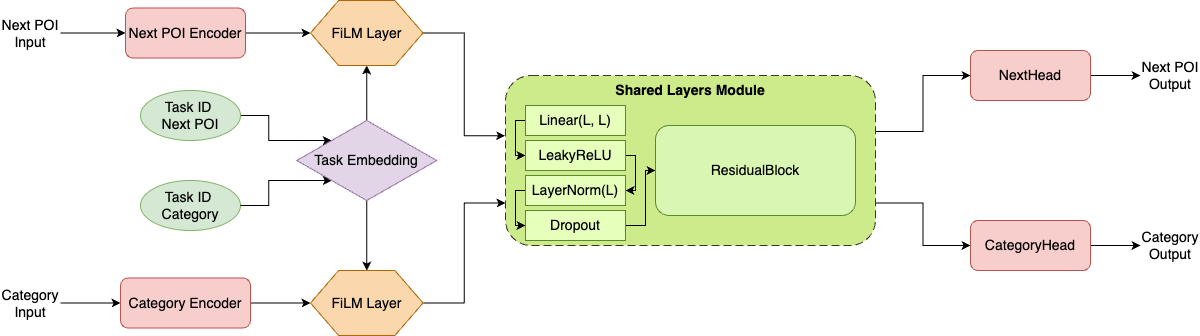
\includegraphics[width=\textwidth]{figures/cbic_mtlnet_arch.png}
    \caption{The proposed Multitask Learning (MTL) architecture. Task-specific encoders process inputs for POI Category Classification and Next-POI Prediction. Feature-wise Linear Modulation (FiLM) layers adapt these features using learnable task embeddings. The modulated representations are then processed by a shared path of residual blocks. Finally, dedicated task-specific heads generate the respective outputs.}
    \label{fig:cbic:arch}
\end{figure}

\subsection{Nash-MTL Optimizer}
\label{sec:cbic:nash}

MTL necessitates a unified update direction that benefits all tasks, even when their gradients conflict. Nash-MTL formulates this as a cooperative $K$-player bargaining game \cite{nash}, where each task acts as an ``agent'' seeking to maximize its utility (loss reduction). The optimizer selects a step that is (i) beneficial to all tasks, (ii) scale-invariant to arbitrary loss re-weightings, and (iii) proportionally fair, ensuring no alternative direction increases one task's utility without decreasing the product of all utilities \cite{nash}. The unique solution satisfying these axioms is the Nash Bargaining Solution (NBS). This approach allows Nash-MTL to ``negotiate'' at each iteration, yielding a compromise descent direction that improves every loss while maximizing the joint progress of the entire system.

\paragraph*{Formal Formulation.}
Given task-specific objectives $\{\mathcal{L}_k(\boldsymbol{\theta})\}_{k=1}^{K}$ and their gradients $\mathbf{g}_k=\nabla_{\!\boldsymbol{\theta}}\mathcal{L}_k$ at current parameters $\boldsymbol{\theta}$, Nash-MTL frames gradient aggregation as a bargaining game to determine the common update direction \cite{nash}. The utility for each task $k$ is its signed improvement, $u_k(\Delta\boldsymbol{\theta})=\mathbf{g}_k^{\!\top}\!\Delta\boldsymbol{\theta}$, where $\Delta\boldsymbol{\theta}$ is the parameter update within an $\varepsilon$-ball \cite{nash}. The NBS is found by maximizing the weighted geometric mean of utilities:
\begin{equation}
\Delta\boldsymbol{\theta}^{*}\;=\;\operatorname*{arg\,max}_{\Delta\boldsymbol{\theta}\in\mathcal{B}_\varepsilon}
\sum_{k=1}^{K}\!\log\!\bigl(u_k(\Delta\boldsymbol{\theta})\bigr)
\quad\text{s.t. }u_k(\Delta\boldsymbol{\theta})>0,\;\forall k.
\label{eq:cbic:nbs}
\end{equation}
By setting $\Delta\boldsymbol{\theta}=\sum_{k}\alpha_k\mathbf{g}_k$ with positive weights $\boldsymbol{\alpha}$, the solution simplifies to solving the nonlinear system $\bigl(\mathbf{G}^{\!\top}\mathbf{G}\bigr)\boldsymbol{\alpha} \;=\; \boldsymbol{\alpha}^{-1}$ \cite{nash}, where $\mathbf{G}=\bigl[\mathbf{g}_1\,\ldots\,\mathbf{g}_K\bigr]$ \cite{nash}. The parameter update is then $\boldsymbol{\theta}^{(t+1)} =\boldsymbol{\theta}^{(t)}-\eta\,\mathbf{G}\boldsymbol{\alpha}$, with $\eta$ chosen to ensure monotonic loss decrease and convergence to a Pareto-stationary point \cite{nash}.

\paragraph*{Practical Aspects.}
Nash-MTL is architecture-agnostic.\footnote{The published sentence continued ``and requires only two
matrix-vector products per iteration''. That cost claim is corrected here rather than reproduced: it
is not supported by the method's own paper, and it understates the cost.} Its invariance to the scale of the individual task gradients, the second of the axioms listed above, balances heterogeneous tasks without manual re-weighting. For efficiency, task weights can be updated less frequently, significantly reducing runtime while maintaining performance~\cite{nash}.
% [round4, REV-020a] Factual correction to reproduced prose. The published sentence read
% "Its reliance on gradient signs rather than scales inherently balances heterogeneous tasks".
% Nash-MTL does not read gradient signs: it is scale-invariant, which is what this same
% chapter states earlier in the same subsection, at :224 ("scale-invariant to arbitrary loss
% re-weightings"). Verified three ways this session: (1) Navon et al., arXiv:2202.01017,
% Axiom 2.4 "Invariance to affine transformation" and Fig. 1 discussion ("Nash-MTL, is
% invariant to changes in loss scale"); the string "sign" appears in that paper only inside a
% bibliography entry for an unrelated method. (2) The CoUrb-era implementation the author
% provided, /Users/vitor/Desktop/mestrado/temp/tarik-new/PoiMtlNet_Novo/src/criterion/
% nash_mtl.py: zero occurrences of sign/abs; get_weighted_loss (:176-232) forms G, computes
% GTG = G G^T (:222), normalizes by its Frobenius norm (:224-227) and solves for alpha
% (:228). (3) This repository's src/losses/nash_mtl/loss.py: same structure at :291-299,
% also zero occurrences of "sign". Claim strength is reduced, not increased: a mechanism
% claim is replaced by the weaker property the paper actually proves. Declared in Table B.1.
% [round5, author decision 1b.3 -- SUPERSEDES the earlier REPORTED-NOT-CORRECTED ruling] The author
% asked for ONE standard: "caso contrario algum revisor pode questionar o fato de alguns erros
% factuais eu alterar o texto e outros nao". The cost claim is now CORRECTED in a footnote and
% recorded in Table~\ref{tab:apx:cbic-errata}, alongside the gradient-scale correction that sits in
% the same published sentence. Evidence: arXiv:2202.01017 does not contain the phrase
% "matrix-vector"; both implementations run an iterative concave-convex procedure, default twenty
% passes, each a convex solve, plus one backward pass per task. The correction runs AGAINST this
% dissertation's interest (it raises the cost of a method the chapter used), which is why applying it
% is the conservative choice as well as the consistent one.

\paragraph*{Parameter Partition.}
In our model (Figure~\ref{fig:cbic:arch}), we explicitly expose two disjoint parameter sets:
\[
  \begin{aligned}
    \Theta_{\text{shared}}   &= \{\texttt{task\_emb},\texttt{film},\texttt{shared\_layers}\},\\
    \Theta_{\text{specific}} &= \{\texttt{category\_encoder},\texttt{next\_encoder},\\
                             &\qquad\ \texttt{CategoryHead},\texttt{NextHead}\}.
  \end{aligned}
\]
This partition enables independent learning-rate scheduling or regularization if domain shifts between tasks emerge during fine-tuning.

The Nash-MTL optimizer was employed for its ability to aggregate tasks gradients in a balanced and principled manner, formulating the optimization process as a bargaining problem and aiming for joint progress across all tasks. In our evaluation, Nash-MTL was compared with different strategies, including PCGrad~\cite{yu2020pcgrad} and an approach with no optimizer. Among these, it was found that Nash-MTL consistently yielded a better overall performance of the MTL model, with a lower combined multitask loss, which supported our decision to adopt it as our choice of optimizer.
